\chapter{Experiments and Evaluation}\label{experiment}

\section{Comparison with Flocking model}

we first simulate the flocking model with various $a_{ij}$ and control laws in Chapter~\ref{flocking} with 2, 3 and 4 agents respectively. The initial position are illustrated in Fig.\ref{fig:simulate_flocking} where only the most front agent has initial velocity pointing forward.
\begin{figure}[htb]
	\centering
	\subfigure[Two agents in a shape of straight line]{\label{fig:2_agents}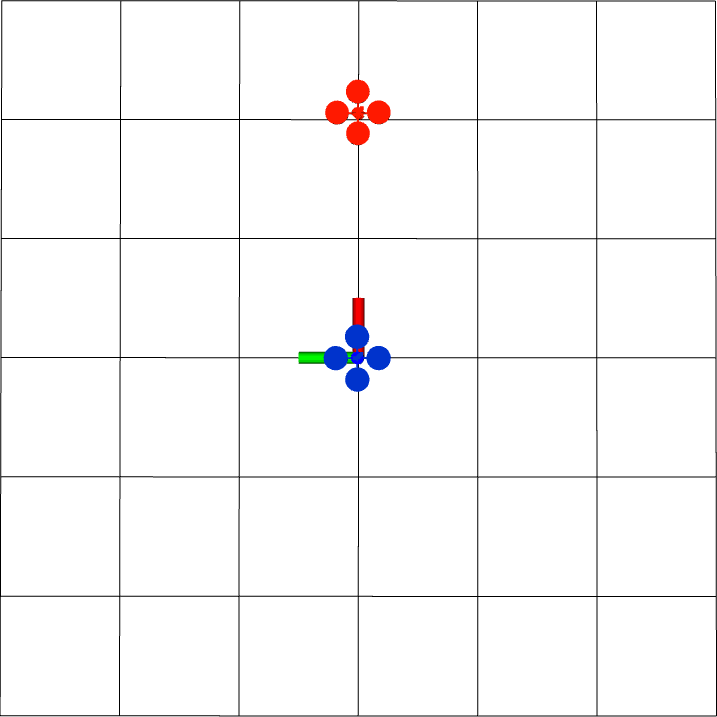
\includegraphics[width=0.31\textwidth]{figure/chapter_5/2_agent.png}}
	\subfigure[Three agents in a shape of equilateral triangle]{\label{fig:2_agents}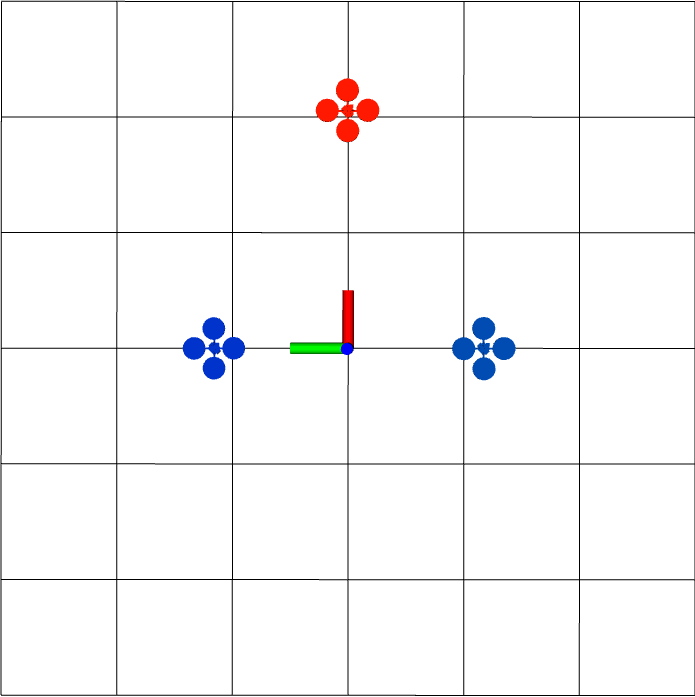
\includegraphics[width=0.31\textwidth]{figure/chapter_5/3_agent.png}}
	\subfigure[Four agents in a shape of diamond]{\label{fig:2_agents}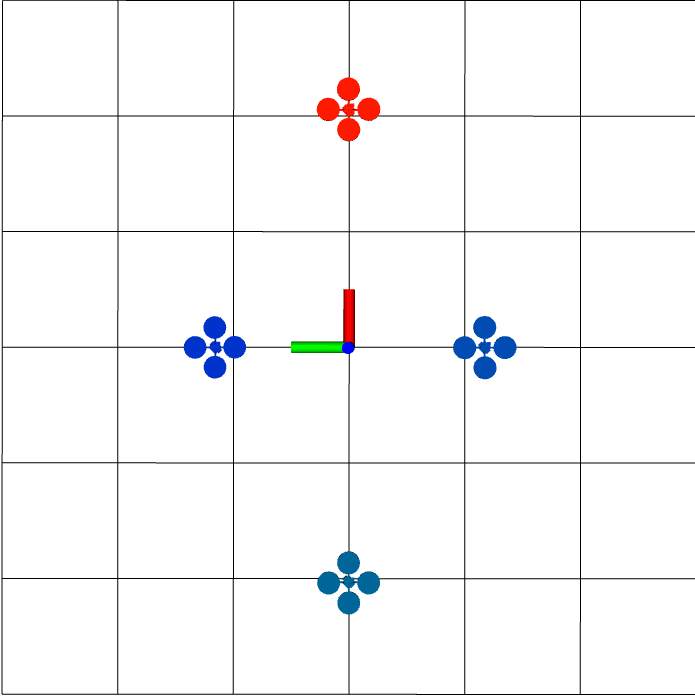
\includegraphics[width=0.31\textwidth]{figure/chapter_5/4_agent.png}}
	\caption{Simulations of multi-UAV flocking}\label{fig:simulate_flocking}
\end{figure}
